\section* {Introduction}
Deep learning opens opportunities in the healthcare sector for several appliances. One of these appliances is image processing in order to detect and predict health conditions \cite{miotto2018deep}.  The initial research focus was the optimization of a deep learning algorithm in predicting pneumonia from x-ray images. Pneumonia is a condition of a lung infection which leads to inflammation inside the air sacs (i.e. alveoli) of the lungs. Pneumonia can unfold to a life-threatening disease.\\ Approximately 450 million cases of pneumonia are recorded every year of which 4 million humans die \cite{ruuskanen2011viral}. Image processing got more accessible in recent years with the upcoming of libraries such as TensorFlow and Keras whose “out-of-the-box” functions already classify images with high accuracy without the need for deeper theoretical knowledge. There are also methods to improve classifiers, which need extensive medical knowledge such as detailed image pre-processing, which exclude non-relevant data (e.g. rib cages) from the image \cite{kulkarnioptimization}, which is not part of this research. However, many medical data sets come with class imbalance. A class of images such as “no condition”, “bacterial infection” or “viral infection” is used to train a supervised deep learning algorithm. \\
Class imbalance can lead to ambiguous predictions and is a problem that has to be addressed before training a deep learning algorithm.  Therefore, our research is focused on how different methods affect the prediction results. This research is focused on the methods, undersampling, oversampling and data augmentation. Figure \ref{fig:plan} shows a schematic overview of the approach pursued in this research.
\begin{figure}[h]
  \centering
  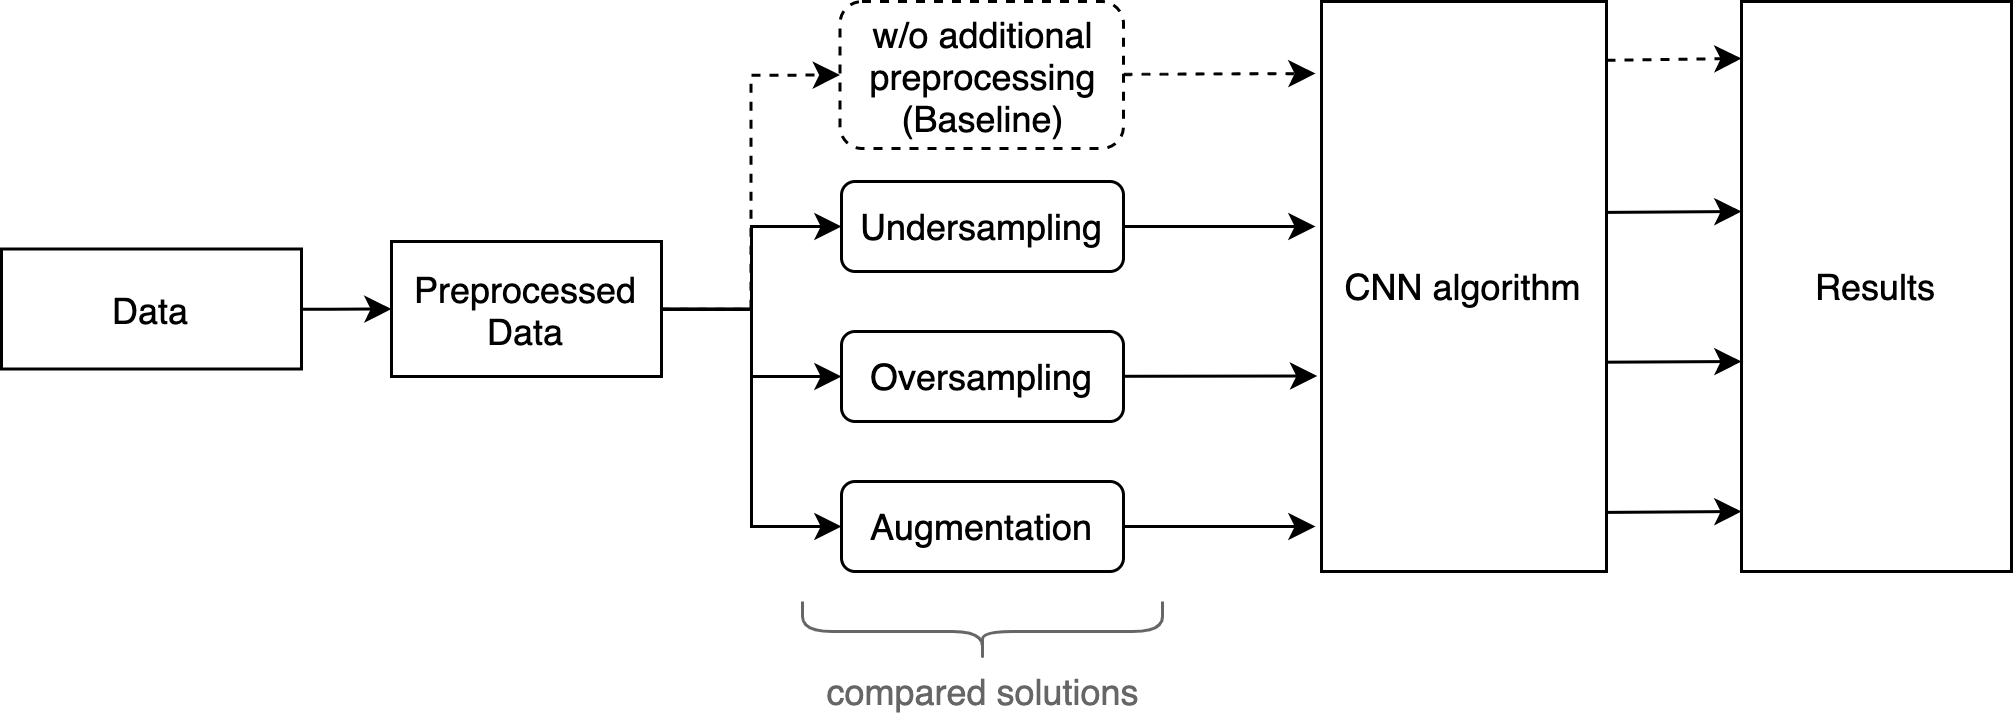
\includegraphics[width=\linewidth]{figures/planOfAttack.png}
  \caption{Way of Proceeding}
  \label{fig:plan}
\end{figure}